\documentclass[12pt]{article}

\usepackage[left=1in,top=1in,right=1in,bottom=1in]{geometry}
\usepackage[utf8]{inputenc}
\usepackage[english]{babel}
\usepackage{graphicx}
\usepackage{csquotes}
\usepackage[
backend=biber,
style=chicago-authordate
]{biblatex}

\usepackage[colorlinks=true,linkcolor=black,citecolor=black,urlcolor=black]{hyperref} 


\usepackage{setspace}
\setstretch{2}

\addbibresource{bibliography.bib}
\AtEveryBibitem{%
  \clearlist{language}%
}
 
\title{Paper Proposal for American Political Development (POLSCI 688)}
\author{Ben Goehring}
\date{\today}

\begin{document}
\begin{titlepage}
\maketitle
\end{titlepage}
\hypersetup{pageanchor=false}


Over the last decade, state governments have passed numerous preemption laws, overturning or preventing municipalities' attempts to increase the minimum wage, ban plastic bags, prevent fracking, protect disadvantaged groups from discrimination, and enact other regulations \parencite{dupuisCityRightsEra2018,schraggerStatePreemptionLocal2017}. While states have preempted local laws in a variety of policy domains, economic regulations have garnered special attention in recent years. In the four year span from 2013 to 2017, 14 states banned localities from raising the minimum wage above the statewide wage; 17 states prevented localities from mandating employers provide some form of paid sick or family medical leave; and 11 states banned localities from requiring government contractors to pay their employees the average local wage \parencite{vonwilpertCityGovernmentsAre2017}.

The recent spate of preemption activity has generated interest among political scientists in the underlying causes of state preemption. Recent studies point to the conservatism of state legislatures \parencite{goodmanStateLegislativeIdeology2019} as well as interest group lobbying and the dominance of Republican parties in state capitals since 2010 as key causes of preemption \parencite{hicksHomeRuleBe2018,fowlerStatePreemptionLocal2019,flavinExplainingStatePreemption2019,riverstone-newellRiseStatePreemption2017}. Scholars have also found relationships between state preemption and the share of African Americans in the population \parencite{flavinExplainingStatePreemption2019} as well as between preemption and legislative professionalism, political culture, and home-rule status \parencite{fowlerStatePreemptionLocal2019}. These studies are an important first step in understanding when and why states preempt local laws. Yet, their narrow focus on post-2010 preemption activity, absence of time series analyses,\footnote{For an exception, see \textcite{goodmanStateLegislativeIdeology2019}.} and lack of appreciation for the role of local action in spurring state preemption render their findings suspect.

I argue in this paper that state preemption must be viewed as another battle in a long-running struggle between cities and states over the bounds of local autonomy. Preemption is neither a new phenomenon nor one that can be properly understood by only studying state actions. As a historic phenomenon, one that dates back to battles over tobacco regulation in the 1980's, preemption deserves to be studied across a time frame wide enough to parse out whether, for instance, it is always the case that conservative Republican state governments are more likely to overturn local regulations or whether such a finding is a product of restricting analyses to a narrow time period. As another instance of cities and states struggling over how much authority cities should possess, preemption needs to also be studied with an eye toward the actions of both states and cities. If preemption is a product of relations between two entities, we cannot fully understand the actions of one without accounting for the actions of the other.

I begin by overviewing the history of preemption and situating it within an even longer history of city-state relations. Next, I provide a framework for testing the underlying causes of preemption. I argue that preemption is most likely to occur when the threat of local action is high, there is significant divergence between the interests of state and local policymakers, and organized interests are mobilized at the state level. Third, I propose to test my theory using data on states' preemption of local ordinances regulating the consumption and sale of tobacco. As I detail below, there is a long history of states' preempting local tobacco policies and high-quality data on local regulations and state tobacco laws. I conclude by discussing some expected findings and implications from my work. 

\subsection*{City-state relations}
State interference in municipal governance dates back to the founding of the United States. Following the passage of the Constitution, which does not mention cities or other types of sub-state municipalities, state legislatures began to exert control over cities chartered in the colonial era in order to reduce local elites' authority. While state intervention was relatively rare in the first half of the 19th Century, states took a much more active role in municipal affairs in the latter half of the century. The challenges wrought by urbanization and industrialization led many reformers and state legislators to see the states as having a necessary role in governing large cities, while concerns over urban corruption and nativist prejudices further galvanized efforts to increase state control over city affairs (\cites[p. 53-57]{bermanLocalGovernmentStates2003}[p. 9]{kraneHomeRuleAmerica2000}). 

Rising political competition at the national and state levels also led to increased state control over municipal affairs. As party competition increased between Democrats and Republicans, state officials increasingly came to see cities as key sources of votes and patronage. As a result, municipal departments often became caught in the middle of partisan fights and were consequently transferred from city to state control --\footnote{delete after the dash and replace with example of NY department in Berman} before being transferred back to city jurisdiction when the other party gained power at the state level (\cites[p. 57-60]{bermanLocalGovernmentStates2003}[p. 11]{kraneHomeRuleAmerica2000}). Municipal employees were also often at the mercy of state legislators, as their salaries and employment status could be changed without cause via legislation \parencite[p. 59]{bermanLocalGovernmentStates2003}.

Around the turn of the century, amid concerns over states' corruption and interference in city governments, progressive reformers began to push for increased local control over municipal governance. What began as a movement to stop legislation targeting specific city policies, personnel, and departments grew into a larger push for increased local autonomy via Home Rule \parencite[p. 11]{kraneHomeRuleAmerica2000}. Home Rule has taken on different forms \parencite{richardsonDillonRuleMars2011}, but its early proponents emphasized that cities should have a degree of immunity from state interference and possess the authority to legislate in areas of local concern (\cites[p. 11-12]{kraneHomeRuleAmerica2000}[p. 1124-1125]{dillerIntrastatePreemption2007}). They hoped that by carving out separate spheres of authority for cities and states, city-state relations could mirror relations between the states and federal government. By the end of the 19th Century, Missouri, California, Washington, and Minnesota had instituted Home Rule, with nine more states following suit in the first 12 years of the 20th Century \parencite[p. 11]{kraneHomeRuleAmerica2000}.

Economic and legal forces limited Home Rule's effect on cities' ability to self-govern. The Great Depression sharply reduced cities' revenues, leading municipalities to seek out assistance and place less emphasis on their independence. As cities were often underrepresented at the state level (\cites{ansolabehereEndInequalityOne2008}[p. 64-67]{bermanLocalGovernmentStates2003}) and slow in providing assistance, city leaders focused much of their attention on building relationships with the federal government \parencite[p. 64-65]{bermanLocalGovernmentStates2003}. The legal structure of Home Rule also reduced its impact on local autonomy. By situating municipal policymaking authority within a separate, local sphere, Home Rule empowered state judges to curtail the bounds of city power (\cites[p. 1125]{dillerIntrastatePreemption2007}[p. 12]{kraneHomeRuleAmerica2000}). Following the legal doctrine of Dillon's Rule, which treats municipal authority as only extending to the policy domains explicitly delegated by the state government, state judges often narrowly construed the bounds of cities' authority, regardless of Home Rule status (\cites[p. 1125]{dillerIntrastatePreemption2007}[p. 71-72]{bermanLocalGovernmentStates2003}).\footnote{Dillon's Rule is named after the 19th Century jurist John Dillon. In an 1868 case in Iowa and treatise on municipal law published five years later, Dillon argued for cities to be treated as subservient to their states. "[Municipalities]," Dillon wrote, "possess no powers or faculties not conferred upon them, either expressly or by fair implication, by the law that creates them, or other statues applicable to them" \parencite[p. 93]{dillonLawMunicipalCorporations1873}. While Dillon's doctrine gained widespread traction, he was not the first to provide a legal justification for cities' subservience to states, James Kent's \textit{Commentaries on American Law}, published in 1836, argued that cities "possess subordinate legislative powers\ldots] subject to the control of the legislature of the state" \parencite[Quoted in ][p. 9]{kraneHomeRuleAmerica2000}}

Home Rule's shortcomings led to another reform movement in the 1950's and 1960's that set the stage for recent decades' state preemption battles. In order to evade state judges' narrow interpretation of local spheres of authority, advocates of municipal autonomy pushed states to allow cities to be able to legislate in any domain that does not conflict with state law \parencite{dillerIntrastatePreemption2007}. Advocates believed that shifting the bounds of local autonomy from the sphere of local concern to the entire domain of policies not in conflict with state law would empower local policymaking and reduce the influence of state judges. While advocates' efforts were largely successful, as a majority of states now use some form of this ``legislative'' Home Rule to structure city-state relations \parencite[p. 1126]{dillerIntrastatePreemption2007}, their vision of expanded local autonomy with limited state interference has not been fully realized. Although legislative Home Rule removed judges' authority to determine whether a city law falls within its local sphere of authority, it gave judges the new power to define whether local laws are in conflict with state law \parencite{dillerIntrastatePreemption2007}. Furthermore, it empowered state legislatures to change state law in order to change the bounds of local autonomy, providing states with the opportunity to explicitly preempt local laws. 

\subsection*{History of preemption}
The emergence of legislative Home Rule in the U.S. states set the stage for the preemption battles of recent decades. Under such a legal regime, cities enjoy expanded authority but face the threat of interference from either state courts or legislatures \parencite{dillerIntrastatePreemption2007,goodmanStateLegislativeIdeology2019}. Court-driven preemption occurs when an interest group, the state, or another plaintiff appeals to a state court that a local law surpasses the city's policymaking authority. While this court-centered form of preemption is important and constitutes a significant share of overall preemption activity \parencite{swansonStateGovernmentPreemption2018,dillerIntrastatePreemption2007}, my focus here is on preemption stemming from the actions of state legislatures. Legislative preemption occurs when a state steps in to explicitly ban local policymaking on a certain topic, such as plastic bags or guns, effectively setting a statewide ceiling on regulation.\footnote{States have also considered but not passed even wider forms of preemption that ban policymaking across expansive policy domains, such as private property, business, and commerce \parencite[p. 2007]{briffaultChallengeNewPreemption2018}.}

Legislative preemption began in earnest in the 1980s over the issue of tobacco regulation \parencite{hicksHomeRuleBe2018,riverstone-newellRiseStatePreemption2017,nationalcancerinstituteStateLocalLegislative2000}. In the mid-1980s, municipalities began to regulate the sale and consumption of tobacco. By 1995, 1,006 local tobacco ordinances existed in the U.S., restricting indoor smoking, minors' ability to purchase tobacco, and tobacco advertising \parencite{siegelPreemptionTobaccoControl1997}. The tobacco industry mobilized in response to the spread of local regulations and pressured states to clamp down on cities' ability to regulate tobacco. Lobbying firms representing the tobacco industry were explicitly supportive of state preemption policies. The Tobacco Institute, for instance, listed tobacco preemption laws as a ``proactive'' goal for 1990; three years later, the group still sought to ``encourage and support statewide legislation preempting local laws'' \parencite[Quoted in][]{centersfordiseasecontrolPreemptiveStateTobaccoControl1999,nationalcancerinstituteStateLocalLegislative2000}. The tobacco industry focused on preempting policies at the state level rather than the fighting local regulations because of the efficiency of advocating for blanket bans and tobacco forces' comparative political advantage. As one lobbyist summed it up, ``The Tobacco Institute and tobacco companies' first priority has always been to preempt the field, preferably to put it all on the federal level, but if they can't do that, at least on the state level, because the health advocates can't compete with me on a state level. They never could. On the local level, I couldn't compete with them" \parencite{skolnickCancerConvertsTobacco1995}.

The tobacco industry succeeded in advocating for laws preempting local tobacco regulations in a number of states. Between 1982 and 1996, 31 states enacted approximately 120 different tobacco-related preemption laws \parencite{centersfordiseasecontrolPreemptiveStateTobaccoControl1999}. Although the number of laws preempting tobacco regulation in certain domains such as indoor smoking in public and private buildings decreased over the following fifteen years, 13 states still preempt at least some local smoke free ordinances \parencite{centersfordiseasecontrolStatePreemptionLocal2010}. In four of those states---Connecticut, Florida, New Hampshire, and South Dakota---all local smoke-free ordinances are preempted \parencite{centersfordiseasecontrolStatePreemptionLocal2010}.\footnote{Some of these states' preemption provisions resulted from court decisions rather than legislative acts. While separating instances of court and legislative preemption is beyond the scope of this paper proposal, I will differentiate the two once I receive the tobacco data.}

Other interest groups noticed the tobacco industry's efforts to prevent local regulations. Working on behalf of firearm enthusiasts and producers, the National Rife Association (NRA) became a key advocate for state laws preempting gun control regulations \parencite{hicksHomeRuleBe2018}. Today, 43 states preempt at least some local regulation of guns and ammunition \parencite{giffordslawcenterPreemptionLocalLawsn.d.,schraggerStatePreemptionLocal2017}, with many of the laws dating back to the 1980s and 1990s. Of the eleven states that do not allow any firearm or ammunition ordinances, for instance, nine of them passed their preemption laws before 2000 \parencite{schraggerStatePreemptionLocal2017}. More recently, some states have adopted gun control preemption laws that impose severe penalties on non-compliant local officials and cities. While such penalties are not exclusively associated with laws preventing local firearm regulation, many of the penalties for not complying with gun preemption laws are especially severe. Kentucky criminalizes non-compliance with the state preemption law, while local officials in Florida can be fined and even removed from office for not complying the state's gun preemption law \parencite{briffaultChallengeNewPreemption2018}.

\textcite{hicksHomeRuleBe2018} posits that, following the expansion of tobacco and gun preemption policies in the 1980s and 1990s, the 2000s saw a decrease in the number of preemption policies passed. While the lack of exhaustive preemption data makes these types of claims difficult to verify, the period did see a slight retrenchment in the number of states with tobacco preemption laws and, compared to the following decade, significantly fewer states preempted local regulations related to labor and earnings \parencite{centersfordiseasecontrolStatePreemptionLocal2010,vonwilpertCityGovernmentsAre2017}. That being said, the period still saw its fair share of preemption activity. Mississippi, Oregon, New Hampshire, and Montana passed legislation preempting at least some forms of local smoke-free tobacco regulations \parencite{centersfordiseasecontrolPreemptiveStateSmokeFree2005}. In addition, in a precursor of the widespread adoption of preemption policies targeting economic regulations after 2010, between 2000 and 2009 eight states prevented local ordinances raising the minimum wage, one state preempted localities from mandating employers offer employees paid family or medical leave and another state preempted localities from requiring government contractors to pay the average local wage \parencite{vonwilpertCityGovernmentsAre2017}.\footnote{Colorado's and Louisiana's laws preempting minimum wage increases date back to 1999 and 1997, respectively. Arizona has prevented localities from requiring government contractors to pay the prevailing wage since 1984 \parencite{economicpolicyinstituteWorkerRightsPreemption2018}.}


\begin{figure}[!ht]
\caption{State preemption of economic and labor ordinances, 1984-2019}
\label{fig:policies}
\centering
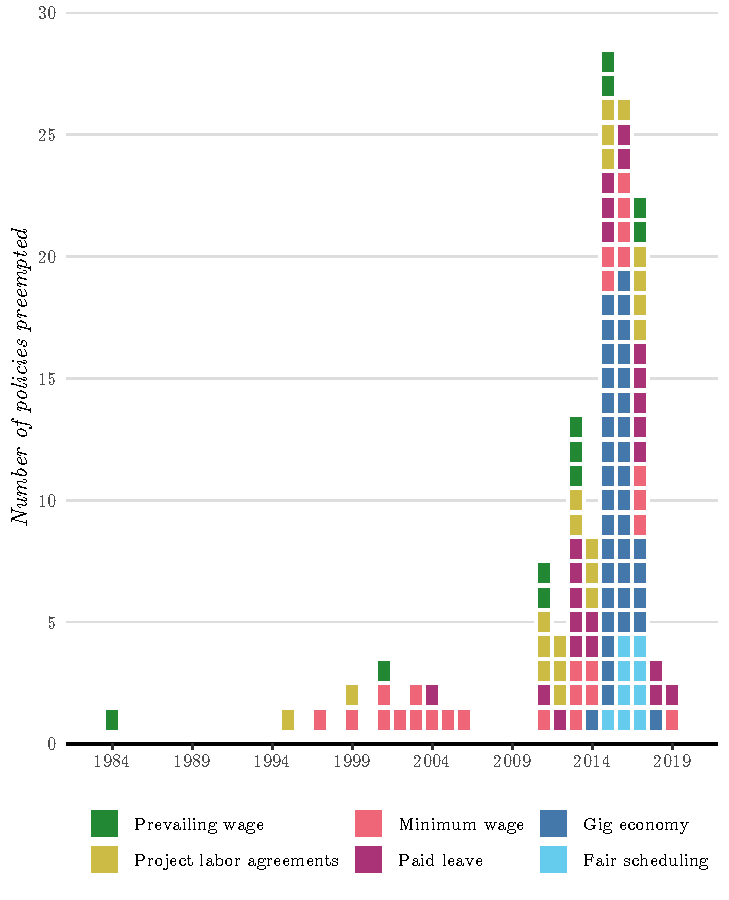
\includegraphics[width=.75\textwidth]{plots/preemption_plot}
\newline\scriptsize{Note: FILL IN. Data collected from, and plot design based on, \textcite{economicpolicyinstituteWorkerRightsPreemption2018}.}
\end{figure}



The roots of state preemption of economic policy regulations lie in . . . 
ALEC? look at recent papers 


\subsection*{Building and testing theories of preemption}
The prior section suggests that preemption has been driven by three actors (localities, states, and interest groups) and their relations to one another. In this section, I drawn upon the history of preemption and the existing literature to develop hypotheses about about when and why we should expect certain relations of cities, states, and interest groups to result in preemption laws. I argue that a state is most likely to preempt a specific municipal regulation when the following three conditions are met:

\singlespacing
\begin{enumerate}
	\item \textit{At least one city in the state is able to pass, or has already passed, the regulation.}
	\item \textit{There is a wide divergence between the policy preferences of the state government and at least one city in the state.}
	\item \textit{Relevant interest groups are organized at the state level.}
\end{enumerate}
\setstretch{2}

The first condition concerns the threat of local policymaking. The states govern their cities using a variety of legal regimes, resulting in variation in local autonomy and the likelihood of municipal policymaking. If institutional rules prevent cities from passing regulations in the first place, states should not be expected to take the time to preempt specific municipal ordinances. The second condition concerns the ideological divide between cities and their states. If cities and states possess different preferences over the given regulatory measure, we should expect states to be more willing to preempt local authority. In states where city and state preferences are closer to one another, states will be more willing to let localities engage in policymaking. Finally, the third condition concerns the activity of relevant interest groups. The narrative above suggests that tobacco lobbying firms, the NRA, and ALEC have played a key role in mobilizing states to clamp down on local policymaking. Where these groups are more powerful, we should see more preemption activity. 

It is tempting to view each of the three conditions as necessary -- that preemption will only occur when all three conditions are met. However, I think this is a bit too strict. It may be the case, for instance, that some states will, following the lead of interest groups, preempt local policymaking even when the threat of local action is low. Nevertheless, I do think that each of the three conditions offers important and distinctive explanatory power, and that their combination provides the highest likelihood of state preemption. It will be important to think more about how the conditions relate to one another as this project progresses.

I hope to show that these conditions should apply to all preemption activity, regardless of the policy area. While the broad applicability of the hypotheses is an advantage, the reality of the data on state preemption and local policymaking means that testing hypotheses across multiple policy domains remains a distant goal. Collecting data on cities' policymaking (which is necessary to test whether the realization of the threat of local action spurs states to act preemptively) is no small task. I only know of one resource, the U.S. Tobacco Control Laws Database (TCLD) maintained by the American Nonsmokers' Rights Foundation,\footnote{\url{https://no-smoke.org/materials-services/lists-maps/}} that tracks both local ordinances and state preemption laws. While collecting data on cities' attempts to pass other regulations is important (especially in the policy areas that have seen the sharpest rise in preemption activity in recent years), my aims are more modest. I hope to use the TCLD's data on local tobacco regulation and state preemption over the past 40 years to test whether my three conditions hold. In the following pages, I provide further justification of the three conditions and offer concrete means of testing them in the context of tobacco preemption. 

\subsubsection*{Hypothesis 1}
The first condition concerns cities' capacity to pass regulations. As described above, cities have often lacked this power. Early formulations of Home Rule, paired with narrow interpretations of cities' sphere of policymaking authority, hindered cities' ability to legislate as they saw fit. Since mid-century, many states have adopted legislative Home Rule regimes that permit a greater degree of state policymaking while allowing state courts and legislatures to intervene and deem local ordinances in conflict with state law. Nevertheless, there still remains considerable variation in the legal regimes governing city-state relations. This patchwork of legal rules results in differences across states in the likelihood of state preemption. In states where Dillon's Rule is still frequently applied by judges, cities possess limited policymaking authority. They can only legislate in policy domains that have been explicitly permitted by the state. While states can theoretically grant wide authority to cities and then preempt ordinances by curtailing city's delegated power, states that employ Dillon's Rule usually delegate narrow powers to cities in the first place. As a result, cities have little capacity to legislate and if they do act outside the scope of their delegated authority, it usually falls to the state courts to determine if the ordinance is legal \parencite{dillerIntrastatePreemption2007}.

In other states, cities' authority is structured according to the earlier formulation of Home Rule. Cities enjoy authority over matters of ``local concern,'' which is left open to judges' interpretation. Consequently, if a city ordinance is preempted, it is usually the result of a court deciding that the city acted outside of its local area of concern \parencite{dillerIntrastatePreemption2007}. In contrast, legislative Home Rule empowers cities to pass any ordinance that does not conflict with state law. While cities enjoy broad authority in such a regime, state legislatures, as discussed above, also possess the authority to intervene and curtail the bounds of local autonomy. Therefore, it is in states that govern cities with legislative Home Rule that we should expect to see the greatest level of preemption activity. 

Unfortunately, given the complexities of state-local relations, there is no clear method for classifying states' legal regimes. Even the distinction between Home Rule and Dillon's Rule has been challenged \parencite{richardsonDillonRuleMars2011}. In a review of different classification schemes, \textcite{dillerIntrastatePreemption2007} notes that some scholars count 48 states with Home Rule while others count 45. Differentiating between the type of Home Rule is even trickier. One study counts 26 states with legislative Home Rule while others argue that the vast majority of Home Rule states employ legislative Home Rule. Moreover, classification disagreements do not only occur at the margin. In their analysis of the causes of state preemption, \textcite{fowlerStatePreemptionLocal2019}, citing \textcite{kraneHomeRuleAmerica2000}, only treat 10 states as using Home Rule. Deciding upon a classification scheme will be a necessary but challenging step as this project progresses.

While states' legal regimes provide one perspective on the threat of local action, another more concrete measure is whether a city in a state has already passed a tobacco regulation. Unlike the legal rules governing cities, which measures the potential for local action, whether a city has already regulated the sale or consumption of tobacco captures the realization of the threat. Controlling for cities' policymaking is notably absent from recent quantitative analyses of preemption \parencite{fowlerStatePreemptionLocal2019,goodmanStateLegislativeIdeology2019,flavinExplainingStatePreemption2019}, likely due to the difficulty of collecting data on cities' policies. Luckily, the TCLD systematically tracks local tobacco regulations alongside states' preemption laws. It includes the tobacco regulations of 98\% of the cities in the U.S. with more than 75,000 inhabitants, allowing me to test my hypotheses across all fifty states.

\subsubsection*{Hypothesis 2}
The second condition contends that diverging policy preferences between the state government and at least one city in the state increases the likelihood of state preemption. Struggles between cities and states over the bounds of local autonomy usually pit conservative state governments against liberal cities \parencite{rapoportBlueCitiesBattle2016,riverstone-newellRiseStatePreemption2017}, although this is not always the case.\footnote{For instance, in 2013, Oregon preempted cities from regulating genetically-modified crops and, in 2017, New York overturned New York City's tax on plastic bags \parencite{mckinleyCuomoBlocksNew2017,scharffHyperPreemptionReordering2018}.} Given the increasing number of state preemption laws targeting local economic regulations and increasing polarization between Republicans and Democrats on economic and labor issues over the past two decades \parencite{grumbachBackwatersMajorPolicymakers2018}, Republican control of government and state conservatism play an unsurprisingly key explanatory role in recent studies of preemption \parencite{hicksHomeRuleBe2018,riverstone-newellRiseStatePreemption2017,flavinExplainingStatePreemption2019,fowlerStatePreemptionLocal2019}. 

While Republican control of government and conservatism certainly correlate with recent preemption activity, we do not yet have a clear idea of whether partisanship and ideology matter in absolute or relative terms. In other words, we do not know whether Republican control of government and conservatism inherently lead to preemption or whether the connection hinges on the relative difference between the preferences and ideology of the state and its cities. Should we expect preemption to be just as likely in North Dakota as in Texas, since they are both conservative states controlled by Republicans? Or does the fact that Texas contains much more progressive municipalities mean that it is more likely to preempt local ordinances? Based on the above discussion of preemption's history, where preemption often seems to occur as a response to local actions, the latter framing seems to be a more precise formulation of the role of partisanship and ideology. It is also more generalizable, as it does not presume that certain parties and ideologies always pursue preemption. 

While treating ideology and policy preferences in relative terms is important, measuring the liberal ideology of cities is difficult, especially over multiple decades. One, albeit imperfect, approach is to use the share of votes earned by Democratic presidential candidates in urban counties. Figure \ref{fig:ideology} uses this approach to display the growing ideological divide between states and cities. The dashed lines in the figure show the share of votes for the Democratic presidential candidate in the three most populous counties in a state divided by the candidate's vote share in the entire state, averaged over all states that supported the Democratic and Republican candidates, respectively. In 1980, the most populous counties in states that supported either the Republican or Democratic candidate supported the Democratic candidate to roughly the same degree as the entire state. Beginning in the mid-1980s, the share of votes dedicated to the Democratic candidate in urban counties began to increase relative to the Democratic candidate's share of votes in the entire state. The divergence is especially pronounced in states that supported the Republican candidate in the election, implying that urban counties in red states are becoming increasingly liberal relative to their states.  

\begin{figure}[!ht]
\caption{Average relative support of Democratic presidential candidate by geography and state partisanship, 1980-2016}
\label{fig:ideology}
\centering
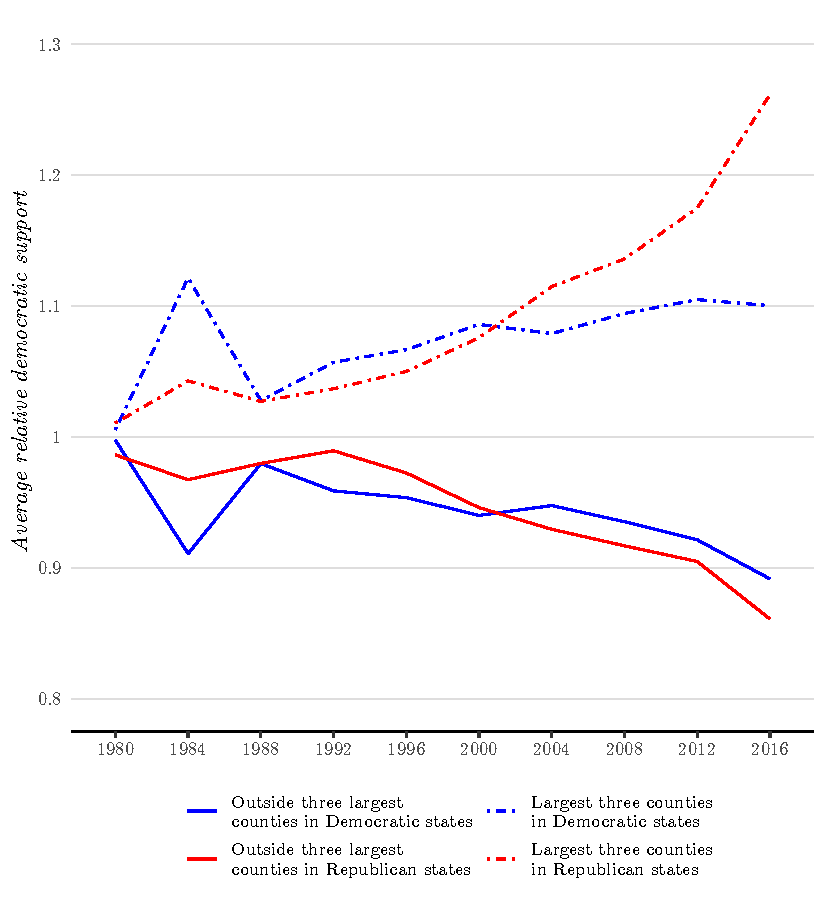
\includegraphics[width=.75\textwidth]{plots/county_support}
\newline\scriptsize{This plot shows the average support for the Democratic presidential candidate in and outside the three largest counties in a state relative to the candidate's support in the rest of the state. For each state and year, the democratic candidate's vote share in and outside each state's three largest counties is divided by his or her vote share in the entire state. Annual average relative support is then calculated, grouping by whether a state supported the Democratic candidate and whether the counties are among the three largest in size. Given time constraints, the total number of votes in a county is used as a proxy for the total population of the county. County-level election returns collected from \textcite{cqpressCQVotingElections2019}.}
\end{figure}

The growing ideological divide between urban and rural areas has been well-documented elsewhere \parencite[e.g.][]{chenUnintentionalGerrymanderingPolitical2013} and cited as a cause of increasing levels of state preemption \parencite{dupuisCityRightsEra2018,hicksHomeRuleBe2018}. As Democratic voters cluster in urban areas, they increase the liberalism of cities relative to states and reduce the number of state-level Republicans representing urban areas. As a result, cities may be more willing to enact more liberal policies that increasingly diverge from the interests of state elected officials, increasing the likelihood that the state will preempt progressive local regulations. In the context of state preemption of tobacco regulations, Figure \ref{fig:ideology} suggests that ideological divergence between rural and urban counties began in the late 1980s, around the time states began to preempt local tobacco ordinances. Interestingly, until about 2000, the ideological gulf between cities and states in states that supported the Democratic presidential candidate was consistently larger than the within-state ideological divide in Republican states. Therefore, if local tobacco regulations occurred in more progressive cities (as measured by support for the Democratic presidential candidate), we might expect to see preemption occurring in both Democratic and Republican states.


Figure \ref{fig:party}, which charts the number of state governments under unified Republican control from 1980 to 2017, also implies that the preemption of tobacco laws may not have been solely driven by the actions of conservative, Republican-controlled governments. The figure shows that just as the 2010s have been a decade of Republican dominance in the states, the 1980s and early 1990s were a period of Democratic control of state governorships and legislatures. Since tobacco preemption began in earnest before Republicans gained widespread power in the states in the 1994 elections, preemption seems to have occurred in many Democratic states. 

The above discussion suggests that we need to move beyond treating Republican control of government and conservative ideology as intrinsically linked to state preemption of local laws. While increasing polarization and diverging preferences between rural and urban areas means that conservative, Republican-controlled states are often the source of recent preemption activity, it does not seem that this has always been the case. The ideological and partisan geography of the U.S. in the late 1980s and 1990s suggests that preemption must have been occurring in Democratic states. It will take getting the TCLD data in-hand for me to determine whether this circumstantial evidence holds up to further scrutiny.

\begin{figure}[!ht]
\caption{Number of state governments under unified partisan control, 1980-2017}
\label{fig:party}
\centering
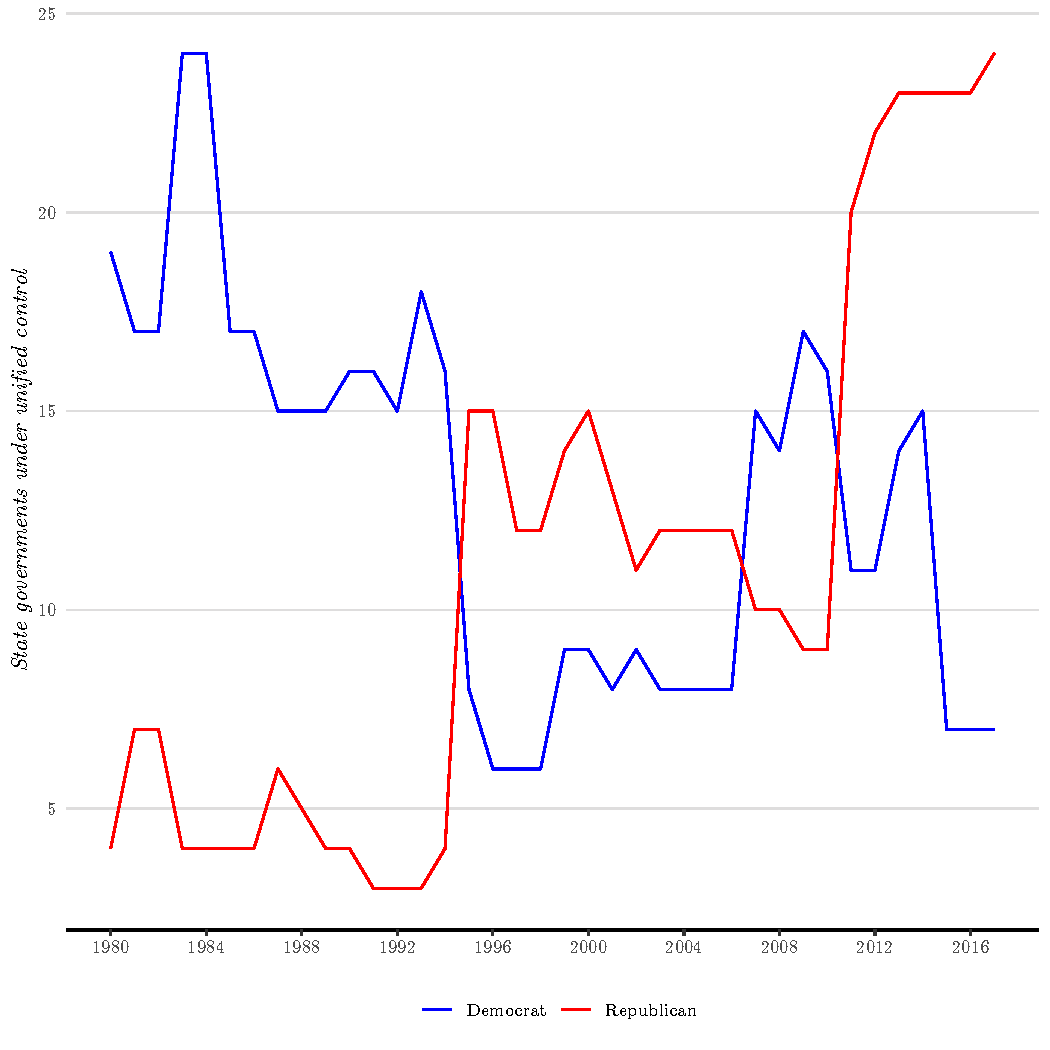
\includegraphics[width=.75\textwidth]{plots/party_control}
\newline\scriptsize{Note: Excludes Nebraska. Sources: \textcite{jordanCorrelatesStatePolicy2017,nationalconferenceofstatelegislaturesStatePartisanComposition2019}.}
\end{figure}

\subsubsection*{Hypothesis 3}
My third and final hypothesis states that preemption is more likely when relevant interest groups are mobilized at the state level. 

\singlespacing
\pagebreak
\printbibliography
 
\end{document}